\section{Численный метод}

Перед тем, как перейти к исследованию полной задачи \ref{matrix_equation} в трёхмерной постановке, рассмотрим одномерное уравнение вида
\begin{equation}
\frac{\partial\vec{u}}{\partial{t}}+\mathbf{A}\frac{\partial\vec{u}}{\partial{x}}=0.
\label{advection_equation}
\end{equation}

\subsection{Решение одномерной задачи}

\subsubsection{Гиперболические свойства определяющей системы уравнений}

Если матрица $\mathbf{A}$ имеет полный набор вещественных собственных значений, 
то такое уравнение называется гиперболическим, и его решения соответствуют 
процессам, которые носят волновой характер. Спектральное исследование матриц $\mathbf{A}_x$, $\mathbf{A}_y$, $\mathbf{A}_z$ проведено в \cite{chelnokov}, где показано, что для них существует полный набор собственных значений и собственных векторов.

В этом случае для любой из матриц $\mathbf{A}_x$, $\mathbf{A}_y$, $\mathbf{A}_z$ существует разложение:
$$\mathbf{A}=\mathbf\Omega^{-1}\mathbf\Lambda\mathbf\Omega,$$
где $\mathbf\Omega$ -- матрица, строки которой $\vec\omega_i^T$ являются собственными для матрицы $\mathbf A$ и
удовлетворяют соотношениям
$$\vec\omega_i^T\mathbf A=\lambda_i\vec\omega_i^T$$ или, что то же самое, транспонированные строки $\mathbf\Omega$ являются собственными векторами для матрицы $\mathbf A^T$
$$\mathbf A^T\vec\omega_i=\lambda_i\vec\omega_i.$$
Здесь $\mathbf\Lambda=diag\{\lambda_i\}$ -- диагональная матрица соответствующих собственных значений.

Домножив уравнение \ref{advection_equation} слева на $\mathbf\Omega$, получаем уравнение
$$\frac{\partial{\mathbf\Omega{\vec u}}}{\partial t}+
\Lambda\frac{\partial{\mathbf\Omega{\vec u}}}{\partial x}=0,$$
которое после перехода к инвариантам Римана ${\vec v}=\mathbf\Omega{\vec u}$ приобретает вид
$$\frac{\partial{\vec v}}{\partial t}+
\Lambda\frac{\partial{\vec v}}{\partial x}=0$$
и тем самым распадается на $n$ одномерных уравнений вида
\begin{equation}
\frac{\partial{v_i}}{\partial t}+\lambda_i\frac{\partial{v_i}}{\partial x}=0.
\label{advection_equation_splitted}
\end{equation}
Таким образом, решение уравнения \ref{advection_equation} представляется в виде
суммы плоских волн, движущихся со скоростями $\lambda_i$.


\subsubsection{Сеточно-характеристический метод}

После перехода к инвариантам Римана получено 9 независимых уравнений переноса вида \ref{advection_equation_splitted}. Рассмотрим уравнение такого вида подробнее. Вдоль характеристических кривых $\Gamma$, таких что
\begin{equation}
\label{characteristics}
\frac{dx}{dt} = \lambda,
\end{equation}
уравнение \ref{advection_equation_splitted} принимает вид 
\begin{equation}
\label{characteristic_equation}
\frac{dv_i}{dt} = 0.
\end{equation}
Таким образом, значения инвариантов Римана переносятся с временного слоя $n$ на временной слой $n+1$ вдоль характеристических кривых $\Gamma$. При этом очевидно, что значения $\lambda_i$ будут разные в зависимости от вида матрицы $\mathbf A$, который определяется используемыми реологическими соотношениями.

\begin{figure}[h]
\center{\includegraphics[width=0.5\textwidth]{eps/gcm-idea.eps}}
\caption{Принципиальная схема сеточно-характеристического метода.}
\end{figure}

Алгоритм поиска значений исходных переменных $\vec u$ в некоторой точке $x_m^{n+1}$ на новом временном слое состоит в следующем. Сначала для матрицы $\mathbf A$ необходимо найти собственные числа $\lambda_i$, которые определяют наклон характеристик \ref{characteristics}, выпущенных из точки $x_m^{n+1}$. После этого для каждой характеристики $\Gamma_i$ можно определить точку $x_{i*}^n$ пересечения с временным слоем $n$.

В точке $x_{i*}^n$ тем или иным способом определяются значения переменных $\vec u_{i*}^n$. Способы реконструкции могут быть различными, в данной работе используется интерполяция по сеточному шаблону на предыдущем временном слое (подробнее см.ниже). По найденным значениям $\vec u_{i*}^n$ вычисляется $i$-ый инвариант Римана $v_{i*}^n$ в точке $x_{i*}^n$. Значение инварианта вдоль $\Gamma_i$ будет перенесено в точку $x_m^{n+1}$ на новом временном слое:
\begin{equation}
v_{im}^{n+1} = v_{i*}^n.
\end{equation}

После того, как в точке $x_m^{n+1}$ описанным образом найдены все 9 инвариантов Римана, можно найти в ней исходные переменные $\vec u$. Так как по определению ${\vec v}=\mathbf\Omega{\vec u}$, то
\begin{equation}
{\vec u}_m^{n+1}=\mathbf\Omega^{-1}{\vec v}_*^n,
\end{equation}
где ${\vec v}_*^n$ -- вектор, составленный из значений $v_{i*}^n$, подсчитанных в соответствующих точках на временном слое $n$. Как описано выше, точки, из которых берутся разные компоненты этого вектора, различны.

\subsubsection{Структурированные и неструктурированные сетки}

\todo{Внятно про структурные и бесструктурные сетки. Для структурных - 1ый и 2ой порядок, гибридизация. Для бесструктурных - аналоги.}
\todo{Внятно про курантовский шаг в случае сеток обоих типов.}

\subsubsection{Восстановление значения на предыдущем временном слое в случае сетки из тетраэдров}

\todo{Про интерполяцию}

\subsubsection{Расчёт внутренних узлов в случае сетки из тетраэдров}



\subsubsection{Расчёт граничных узлов в случае сетки из тетраэдров}

\todo{Внятно написать эти два раздела}

\subsubsection{Расчёт контактных узлов в случае сетки из тетраэдров}

Метод, описанный в предыдущем пункте, годится лишь для расчёта внутренних узлов
сетки, т.е. только в том случае, если характеристика, выпущенная из узла, не
выводит за пределы области интегрирования. В случае, когда узел является
внешним, применяется иной подход для решения задачи. Рассматриваемая система
уравнений в граничных узлах области интегрирования имеет не больше трёх
\cite{chelnokov} выводящих характеристик, поэтому для корректной постановки
задачи требуется задание граничных условий для каждого внешнего узла сетки в
количестве, равном числу выводящих характеристик. Граничные условия могут быть
нескольких видов (символы без волны -- для первого тела, с волной -- для второго):
\begin{itemize}
\item{свободная граница
\begin{eqnarray}
\sigma_\tau=\sigma_n=0; \nonumber
\end{eqnarray}}
\item{скольжение тел друг относительно друга 
\begin{eqnarray}
v_n=\tilde{v}_n,\nonumber\\
\sigma_n=\tilde{\sigma}_n,\nonumber\\
\sigma_\tau=\tilde{\sigma}_\tau=0; \nonumber
\end{eqnarray}}
\item{слипание тел
\begin{eqnarray}
v_n=\tilde{v}_n,\nonumber\\
v_\tau=\tilde{v}_\tau.
\end{eqnarray}}
\end{itemize}
В случае, когда узел имеет выводящие характеристики, решение определяется
следующим образом: те компоненты искомого вектора $v^T$, которые не имеют
выводящих характеристик, считаются при помощи сеточно"=характеристического
метода, описанного ранее; остальные уравнения заменяются граничными
соотношениями. После этого, решается полученная СЛАУ, из которой определяются
значения всех компонент вектора $v^T$ в текущем узле.


\subsection{Решение многомерной задачи}

\subsubsection{Схема с расщеплением по направлениям}

Система \ref{matrix_equation} (или что то же самое \ref{matrix_equation_generalized}) позволяет построить схему для решения трёхмерной задачи, если построены и исследованы одномерные схемы для задач:
\begin{equation}
\frac{\partial\vec{u}}{\partial{t}} + \mathbf{A}_{\xi_j} \frac{\partial\vec{u}}{\partial{\xi_j}} = 0.
\end{equation}

Такой подход называется расщеплением по направлениям и был предложен Р.П. Федоренко (\cite{fedorenko}). Идея метода решения исходной задачи состоит в замене исходной системы уравнений \ref{matrix_equation} одномерными системами -- тремя в случае отсутствия в исходной системе правой части и четырьмя, если правая часть имеется:
\begin{equation}
\frac{\partial}{\partial t}\vec u+\mathbf{A}_x \frac{\partial}{\partial x}\vec u
= 0,
\label{matrix_equation_x}
\end{equation}
\begin{equation}
\frac{\partial}{\partial t}\vec u+\mathbf{A}_y \frac{\partial}{\partial y}\vec u
= 0,
\label{matrix_equation_y}
\end{equation}
\begin{equation}
\frac{\partial}{\partial t}\vec u+\mathbf{A}_z \frac{\partial}{\partial z}\vec u
= 0,
\label{matrix_equation_z}
\end{equation}
\begin{equation}
\frac{\partial}{\partial t}\vec u = \vec f.
\label{matrix_equation_f}
\end{equation}

Обозначим $F(\mathbf A_{\xi_1}, \mathbf A_{\xi_2}, \mathbf A_{\xi_3}, \vec f)$ оператор перехода между временными слоями $n$ и $n+1$, а $F_j(\mathbf A_{\xi_j}), j=1..3$ и $F_j(\vec f), j=4$ -- оператор, соответствующий $j$-ому уравнению в расщеплённой системе.

Необходимо сконструировать оператор $F$ из операторов $f_j, j=1..4$, обеспечив при этом аппроксимацию и устойчивость итоговой схемы, а также приемлемую вычислительную сложность алгоритма при его реализации.

Как разобрано выше, для каждой одномерной задачи существует ограничение на шаг по времени
\begin{equation}
\tau_j \le \frac{\min(h)}{\max(|\lambda_j|)},
\end{equation}

где $\min(h)$ -- минимальная высота тетраэдра в сетке, а $\max(|\lambda_j|)$ -- максимальное по модулю собственное число матрицы $\mathbf A_{\xi_j}$. Теоретически, в этом соотношении можно заменить $\min(h)$ на $\min(h_j)$ -- минимальное расстояние в направлении $j$-ой оси координат от узла сетки до точки пересечения с ближайшей гранью соседнего тетраэдра. Это расстояние может быть несколько больше, чем абсолютный минимум высоты по сетке $\min(h)$, и за счет этого обеспечивать несколько больший допустимый шаг по времени. Однако, на практике в силу случайной ориентации как тетраэдров сетки, так и координатных осей, потенциальное преимущество мало и не стоит того, чтобы усложнять алгоритм расчёта как логически из-за добавления новых элементов, так и вычислительно из-за необходимости постоянно определять новые точки пересечения.

При выполнении условия на $\tau_j$ схема, соответствующая оператору $F_j$, устойчива и имеет свой порядок аппроксимации по времени и пространству для одномерной задачи. Теперь рассмотрим различные варианты составления оператора $F$ из $F_j$.


\subsubsection{Схема с расщеплением первого порядка}

В простейшем случае можно сложить операторы $F_j$ с коэффициентами $a_j$. При таком подходе получаем:
\begin{eqnarray}
F(\mathbf A_{\xi_1}, \mathbf A_{\xi_2}, \mathbf A_{\xi_3}, \vec f) = \sum\limits_{j} a_j F_j(\frac{1}{a_j} \mathbf A_{\xi_j}), \nonumber\\
\sum\limits_{j} a_j = 1, \nonumber\\
a_j > 0.
\end{eqnarray}

Такая схема обеспечивает первый порядок аппроксимации итогового оператора $F$, если в качестве $F_j$ были выбраны схемы как минимум первого порядка. В выборе $a_j$ присутствует определённый произвол, что позволяет использовать их для получения максимального шага по времени.

Действительно, собственные числа матриц $\mathbf A_{\xi_j}^* = \frac{1}{a_j} \mathbf A_{\xi_j}$ будут в $a_j$ раз отличаться от собственных чисел исходных матриц $\mathbf A_{\xi_j}$. Максимально допустимый шаг по времени
\begin{equation}
\tau \le \max{\tau_j} = \frac{\min(h)}{\max(|\lambda_j^*|)} = \frac{\min(h)a_j}{\max(|\lambda_j|)}.
\end{equation}

Таким образом, для максимизации допустимого шага получаем условие:
\begin{equation}
\frac{a_1}{\max(|\lambda_1|)} = \frac{a_2}{\max(|\lambda_2|)} = \frac{a_3}{\max(|\lambda_3|)}.
\end{equation}

Откуда следует
\begin{eqnarray}
a_j = \frac{\max(|\lambda_j|)}{\max(|\lambda_1|)+\max(|\lambda_2|)+\max(|\lambda_3|)},\nonumber\\
\tau = \frac{\min(h)}{\max(|\lambda_1|)+\max(|\lambda_2|)+\max(|\lambda_3|)}
\end{eqnarray}

Видно, что при таком конструировании расщепления получается вычислительно простой алгоритм -- требуется только вычислить независимое воздействие операторов $F_j$ на временном слое $n$, чтобы потом получить значение на временном слое $n+1$ как их сумму. Однако, схема обеспечивает только первый порядок аппроксимации $F$, даже если отдельно $F_j$ имеют более высокий порядок. Кроме того, допустимый шаг по времени заметно уменьшается (как правило, в 3 раза, так как $\max(|\lambda_j|)$ одинаково для всех матриц $\mathbf A_{\xi_j}$.


\subsubsection{Схема с расщеплением второго порядка}

Для обеспечения второго порядка аппроксимации итоговой схемы необходимо операторы $F_j$ не сложить, а перемножить
\begin{eqnarray}
\label{split_scheme_2nd_order}
F(\mathbf A_{\xi_1}, \mathbf A_{\xi_2}, \mathbf A_{\xi_3}, \vec f) = F_1(\mathbf A_{\xi_1}) F_2(\mathbf A_{\xi_2}) F_3(\mathbf A_{\xi_3}).
\end{eqnarray}

С точки зрения реализации это означает, что сначала к значениям на временном слое $n$ применяется первый оператор, потом к результату действия первого оператора -- второй, к результату второго -- третий. Значения, полученные после применения всех операторов, являются значениями на новом временном слое $n+1$:
\begin{eqnarray}
\vec u^{'} = F_1(\mathbf A_{\xi_1}) \vec u^n, \nonumber\\
\vec u^{''} = F_2(\mathbf A_{\xi_2}) \vec u^{'}, \nonumber\\
\vec u^{n+1} = F_3(\mathbf A_{\xi_3}) \vec u^{''}.
\end{eqnarray}

Допустимый шаг по времени определяется минимальным допустимым шагом по времени для схем $F_j$:
\begin{eqnarray}
\tau = \min\limits_{j}(\tau_j) = \min\limits_{j}(\frac{\min(h)}{\max(|\lambda_j|)}) = \frac{\min(h)}{\max\limits_{j}\max(|\lambda_j|)}.
\end{eqnarray}

Таким образом, расщепление данного вида обеспечивает второй порядок аппроксимации и не приводит к уменьшению допустимого шага по времени. Однако, если использовать схему в виде \ref{split_scheme_2nd_order}, то очевидным образом возникает несимметрия решения, так как направления координатных осей перестают быть равноправными.

Метод симметризации схемы достаточно очевиден -- необходимо использовать не одно произведение операторов, которое порождает выделенные направления, а усреднять все возможные перестановки операторов $F_j$:
\begin{eqnarray}
\label{split_scheme_2nd_order_sym}
F(\mathbf A_{\xi_1}, \mathbf A_{\xi_2}, \mathbf A_{\xi_3}, \vec f) = \frac{1}{6} \sum\limits_{i \ne j \ne k} F_i(\mathbf A_{\xi_i}) F_j(\mathbf A_{\xi_j}) F_k(\mathbf A_{\xi_k}).
\end{eqnarray}

Такая схема становится симметричной, но теперь приходится считать действие операторов $F_j$ 18 раз вместо 3 раз.


\subsubsection{Схема с расщеплением и случайным выбором базиса}

Альтернативным способом симметризации схемы \ref{split_scheme_2nd_order} является случайный выбор базиса. В этом случае схема расщепления обеспечивает второй порядок аппроксимации многомерной задачи и возможность использовать большое значение $\tau$. Случайный выбор базиса обеспечивает отсутствие выделенных направлений и симметричность решения. За счет этого на каждом временном шаге требуется вычислять только 3 оператора $F_j$.

Обратной стороной такого подхода, который проявляется при практической реализации метода, является тот факт, что в случайно выбранном базисе из-за изменения направлений осей постоянно меняются точки на предыдущем временном слое, в которые попадают характеристики и по которым производится реконструкция решения. В результате требуется искать эти точки заново после смены базиса на каждом шаге. Однако, при разумной организации структур данных для хранения сетки, вычислительная сложность этой операции достаточно невелика и такой подход оказывается значительно экономичнее, чем вычисление операторов $F_j$ дополнительные 15 раз.


\subsection{Движение сетки}

\todo{Переписать слова ниже. Объяснить внятно про конвективные члены.}

В случае конечных деформаций существует несколько подходов к описанию движения точек среды.

Эйлерова сетка строится однократно и в дальнейшем не изменяется. Это может быть наилучшим решением для тел с фиксированными границами. Для решения задач с конечными деформациями границ выбирают наиболее простую форму эйлеровой сетки — декартову решетку, потому что, независимо от формы ячеек, неподвижные узлы и ребра сетки не будут совпадать в каждый момент времени с движущимися границами, и неизбежны сложности, описанные для декартовых решеток.

Точки лагранжевой сетки смещаются вместе с точками тела, поэтому границы тела всегда совпадают с сеточными линиями. Однако при наличии сдвиговых деформаций в теле, ячейки лагранжевой сетки могут постепенно вырождаться и пересекать друг друга. Численные методы при вырождении сетки обнаруживают неустойчивость и счет приходится прекращать. Поэтому неизбежен подход, называемый лагранжева сетка с перестройкой, в котором, как только детектируется приближение сетки к вырожденному состоянию, производится построение новой сетки, а значения в новых узлах интерполируются из прежних значений. Процедура интерполяции сама по себе приводит к потере точности решения, поэтому желательно перестраивать сетку как можно реже. Ниже будет предложен альтернативный способ решения проблемы больших деформаций, который вместо перестроения сетки использует динамический выбор сеточного шаблона в зависимости от локальных свойств решения.

Подвижная сетка является обобщением лагранжевой, ее точки движутся от слоя к слою с ненулевыми скоростями и смещаются как относительно неподвижной системы координат, так и относительно точек тела. Их движение может быть подобрано таким образом, чтобы исключить вырождение сетки со временем. Однако использование подвижной сетки требует вносить изменения в решаемые уравнения для учета конвективных членов.

Расчет на лагранжевой сетке из тетраэдров подразумевает, что скорость смещения вершин сетки совпадает со скоростью среды. Но в методах второго порядка и выше вводятся дополнительные узлы, отличные от вершин, движение которых задается линейной интерполяцией движений вершин тетраэдра, в котором они расположены. Даже если скорость всех вершин является лагранжевой, то узлы, не совпадающие с вершинами, смещаются относительно точек среды. Это означает, что при их расчете необходимо учитывать конвективные члены. Отличие скорости этих узлов от скорости среды невелико: $O(h^2)$, где $h$ — мелкость сетки. Собственные значения матриц при поправке на конвекцию также изменятся на $O(h^2)$.

Отличие мест пересечения характеристики до и после поправки со слоем $t^n$ составит $\tau O(h^h2) = O(\tau^3)$, такого же порядка и отличие в восстанавливаемом интерполяцией решении. Поэтому в методе второго порядка можно не рассматривать отличие движения узлов в центре ребер от лагранжевых — это не понизит степень аппроксимации, а в методах третьего порядков и выше поправка необходима.


\subsection{Выделение контактных границ}

При взаимном движении тел, а также в задачах с конечными деформациями отдельной задачей становится построение алгоритма явного выделения контактных границ. Стандартный подход (именно он использован в этой работе) к реализации состоит из двух этапов:
\begin{itemize}
	\item грубое (см. рис. \ref{pic:collision_detection}) определение областей потенциально возможного контакта при помощи AABB\footnote{AABB (Axis-aligned bounding box) -- ограничивающий параллелепипед, выровненный по осям };
	\item уточнение контактирующих узлов внутри найденных областей.
\end{itemize}
\begin{figure}[htp]
\centering
\includegraphics[width=0.6\textwidth]{eps/collision_detection.eps}
\caption{Использование AABB для грубого определения областей контакта. На
рисунке изображены тела $B_1$ и $B_2$, а также AABB, построенные для контуров
$C_1$ и $C_2$ этих тел. Контакты ищутся в пересечении разных AABB.}
\label{pic:collision_detection}
\end{figure}
По пересечению AABB определяются пары <<потенциально>> находящихся в контакте тел. Затем для каждой найденной пары проводится уточнение зоны контакта: проверяются <<на контакт>> все пары узлов одного тела и треугольников поверхности другого. Пары <<контактирующих>> узлов и треугольников определяются полным перебором по <<кандидатов>>, попавших внутрь пересечения AABB. Под контактом точки и треугольника здесь понимается следующее: считаем, что треугольник и точка контактируют, если зона влияния (сфера заранее выбранного радиуса) точки пересекает треугольник (см. рис. \ref{pic:contact_detection}).
\begin{figure}[htp]
\centering
\includegraphics[width=0.6\textwidth]{pdf/contact_detection.pdf}
\caption{Определение контакта.}
\label{pic:contact_detection}
\end{figure}
Если треугольник и точка находятся в контакте, то следующим шагом строится парный виртуальный узел -- этот узел лежит внутри контактирующего треугольника так, чтобы прямая проходящая через реальный и виртуальный узлы, являлась нормалью к треугольнику (см. рис. \ref{pic:contact_processing}).
\begin{figure}[htp]
\centering
\includegraphics[width=0.6\textwidth]{pdf/contact_processing.pdf}
\caption{Построение виртуальных узлов при обработке контактирующих границ.}
\label{pic:contact_processing}
\end{figure}
После того, как виртуальный узел построен, получаются значения всех величин в нём. Для этого в данной работе использовалась линейная интерполяция при помощи барицентрических координат. Задача заключается в следующем (см. рис. \ref{pic:triangle_interpolation}): есть треугольник и точка, лежащая в его плоскости, в трёхмерном пространстве, нужно, используя известные значения в вершинах треугольника, определить значение в точке.
\begin{figure}[htp]
\centering
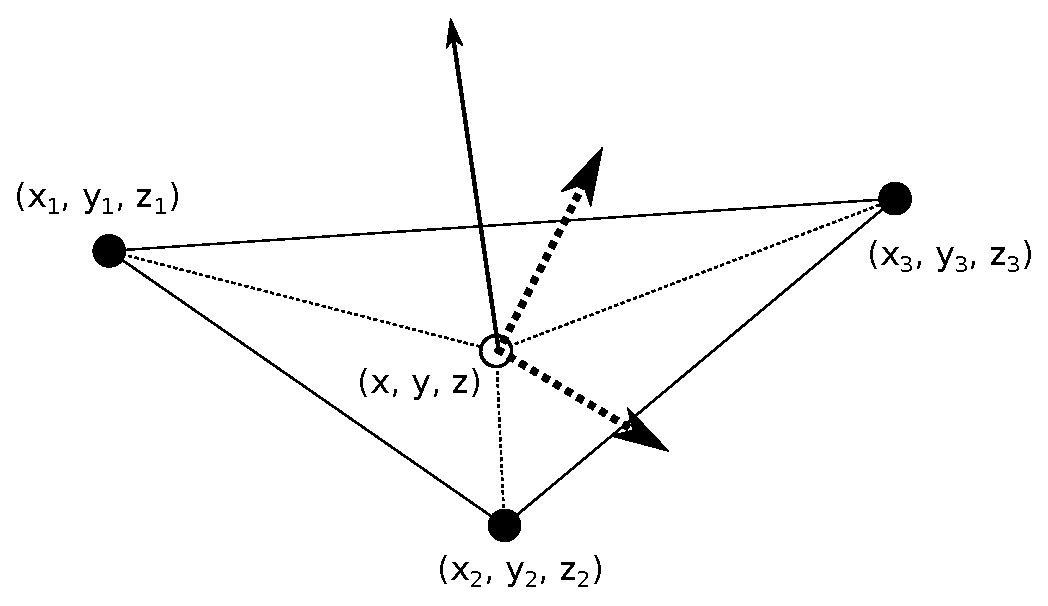
\includegraphics[width=0.6\textwidth]{eps/triangle_interpolation.eps}
\caption{Выбор новых осей координат при интерполяции в треугольнике.}
\label{pic:triangle_interpolation}
\end{figure}
В работе используется следующий подход для реализации интерполяции:
\begin{itemize}
	\item поворотом осей координат добиваемся того, чтобы все четыре точки имели одинаковую координату $\tilde{x}$;
	\item используем интерполяцию в плоскости через барицентрические координаты.
\end{itemize}
Пусть $\vec{n}=(n_1,n_2,n_3)$ -- нормаль к плоскости треугольника, тогда в системе координат с базисными векторами:
\begin{eqnarray}
\label{eq:new_coords}
\vec{\tilde{e}}_1=(n_1, n_2, n_3), \nonumber \\
\vec{\tilde{e}}_2=(n_3, 0, -n_1), \nonumber \\
\vec{\tilde{e}}_3=(n_1*n_2, -n_1^2-n_3^2, n_2*n_3)
\end{eqnarray}
все четыре точки имеют одинаковую координату $\tilde{x}$. Такую систему
координат невозможно использовать, если $n_1=n_3=0$, но в этом случае все точки
имеют одинаковую координату $y$, поэтому, сделав замену
\begin{eqnarray}
\label{eq:new_coords_2}
\tilde{x}=y \\
\tilde{y}=x \nonumber \\
\tilde{z}=z,
\end{eqnarray}
придём опять к ситуации, когда все четыре точки имеют одинаковую координату $x$.
После этих преобразований значение в точке $(x,y,z)$ может быть вычислено по формуле
\begin{equation}
\label{eq:triangle_interpolation}
v=v_1*\lambda_1+v_2*\lambda_2+v_3*\lambda_3, 
\end{equation}
где $v_1,v_2,v_3$ -- значения в вершинах треугольника, а $\lambda_1,\lambda_2,\lambda_3$ -- барицентрические координаты
\begin{eqnarray}
\label{eq:barycentric_coords}
\lambda_1=\frac{(y_2-y_3)(x-x_3)+(x_3-x_2)(y-y_3)}{(y_2-y_3)(x_1-x_3)+(x_3-x_2)(y_1-y_3)}, \nonumber \\
\lambda_2=\frac{(y_3-y_1)(x-x_3)+(x_1-x_3)(y-y_3)}{(y_2-y_3)(x_1-x_3)+(x_3-x_2)(y_1-y_3)}, \nonumber \\
\lambda_3=1-\lambda_1-\lambda_2.
\end{eqnarray}
Эта интерполяция обладает первым порядком точности, что согласуется с порядком точности остальных частей алгоритма.
